% Slides for 2025-04-08
% To create a slide, use the following:
% \begin{frame}{TITLE}
%     BODY
% \end{frame}

% To create a slide with a bullet list, use the following:
% \begin{frame}{TITLE}
%     \begin{itemize}
%         \item ITEM 1
%         \item ITEM 2
%     \end{itemize}    
% \end{frame}

% To create a slide with numbered list, use the following:
% \begin{frame}{TITLE}
%     \begin{enumerate}
%         \item ITEM 1
%         \item ITEM 2
%     \end{enumerate}
% \end{frame}

% To create a slide with a graphic:
% 1. Add the graphic to this folder (named picture.png)
% 2. Use the following:
% \begin{frame}{TITLE}
%     \centering
%     \includegraphics[height=0.7\textheight,width=0.7\textwidth,keepaspectratio]{picture.png}
% \end{frame}

% To create a slide with two columns, use the following:
% \begin{frame}{TITLE}
%     \begin{columns}
%         \begin{column}{0.5\textwidth}
%             COLUMN 1 BODY
%         \end{column}
%         \begin{column}{0.5\textwidth}
%             COLUMN 2 BODY
%         \end{column}
%     \end{columns}
% \end{frame}

\begin{frame}{Data Aug: BG Noise}
    \begin{columns}
        \begin{column}{0.5\textwidth}
            \centering
            \begin{tabular}{c|c}
                alpha range & cmap \\
                \hline \\
                No aug & 0.3746 \\
                0.01-0.02 & 0.3663 \\
            \textbf{0.1-0.2} & \textbf{0.3771} \\
                0.2-0.3 & 0.3492 \\
                \dots & \dots \\
                0.9-0.99 & 0.051
            \end{tabular}
        \end{column}
        \begin{column}{0.5\textwidth}
            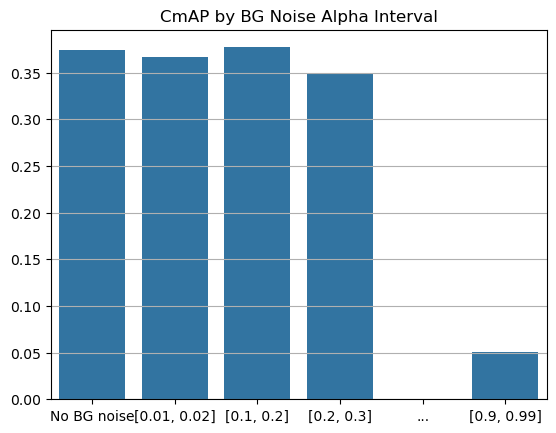
\includegraphics[width=\textwidth]{images/cmap_by_bgnoise.png}
        \end{column}
    \end{columns}
\end{frame}

\begin{frame}{Pipeline Redesign}
    \begin{itemize}
        \item Current pipeline has many errors
        \item Difficult to use
        \item Issues with data preprocessing
    \end{itemize}
    \begin{center}
        \textbf{Goal: Motivate and guide redesign with experiments}
    \end{center}
\end{frame}


\begin{frame}{Desktop App Updates}
    \begin{itemize}
        \item Main focus this quarter on Database Development
        \item Frontend mostly done - fixing bugs and integrating with Backend
        \item Backend working database and inference script
        \item Siya leading CSE 145 group running inference in Rust
    \end{itemize}    
\end{frame}

\begin{frame}{TinyML Updates}
    \begin{itemize}
        \item CSE 145 two groups: Hardware and Software
        \item Hardware: focusing on implementing MCUNET tinyEngine 
        \item Software: focusing on implementing MCUNET tinyNAS
    \end{itemize}    
\end{frame}